\chapter{THI CÔNG HỆ THỐNG ĐIỆN}
\section{Các thiết bị điện}

\subsection{Tổng quan về các phần tử điện}
Để hệ thống hoạt động được luôn cần phần điện. Hệ thống điện chịu trách nhiệm cung cấp nguồn điện, điều khiển các thiết bị trong kết cấu máy như động cơ, driver.
\begin{center}
	\begin{figure}[ht]
	\begin{center}
		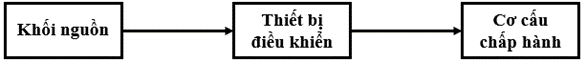
\includegraphics[scale=1]{Chapters/Chapter4/Images/Sodokhoidien}
	\end{center}
	\caption{Sơ đồ các khối trong hệ thống điện}
	\label{fig:sodokhoidien}
	\end{figure}
\end{center}

\subsection{Khối nguồn}
Khối nguồn là bộ phận cung cấp năng lượng cho toàn bộ hệ thống điện trong hệ thống. Để các bóng đèn và động cơ hoạt động ổn định nên nguồn cấp phải đảm bảo điều kiện điện áp và dòng điện luôn ổn định.

Ta lựa chọn nguồn tổ ong.
\begin{figure}[htp]
	\centering
	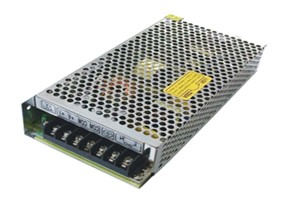
\includegraphics[scale=1]{Chapters/Chapter4/Images/Nguontoong}
	\caption{Nguồn tổ ong}
	\label{fig:Nguontoong}
\end{figure}

Để lựa chọn bộ nguồn phù hợp, phải chú ý đến các thiết bị sử dụng trong mạch điện. Dựa vào thông số về điện áp và dòng điện yêu cầu trên các linh kiện điện để có thể lựa chọn nguồn nuôi thích hợp. Dưới đây là một số linh kiện điện tử và điện áp yêu cầu của các linh kiện đó:
\begin{table}[H]
\centering
\begin{tabular}{|c|c|c|}
\hline 
Linh kiện & Số lượng & Thông số nguồn cấp \\ 
\hline 
LED công suất 3W & 12 & $ 4.2V $ \\ 
\hline 
Driver TB6600 & 3 & $ 12V $ \\ 
\hline 
Động cơ bước & 3 & $ 12V $ \\ 
\hline 
Module L298N & 4 & $ 12V $ \\ 
\hline 
TCA9548A & 1 & $ 5V $ \\ 
\hline 
PCA9685 & 1 & $ 5V $ \\ 
\hline 
\end{tabular} 
\caption{Thông số nguồn cấp cần thiết của các phần tử điện}
\label{tab:nguoncap}
\end{table}

Các thiết bị điện trong máy có dải điện áp hoạt động từ $ 3.8V \sim 12V $.

Cường độ dòng điện cần thiết cho bóng đèn hoạt động: $ 0.789A \times 12 = 9.47(A) $

Cường độ dòng điện cần thiết cho 3 động cơ STEP: $ 0.5A \times 3 = 1.5(A) $

Tổng cường độ dòng điện định mức cần thiết để hệ thống hoạt động bình thường: 
\begin{align*}
9.47A + 1.5A \approx 11A
\end{align*} 

Bộ nguồn được chọn cần có điện áp cung cấp $ 12V $ và dòng điện định mức lớn hơn $ 11A $. Để thuận lợi cho việc nâng cấp hệ thống điện sau này và đảm bảo hệ thống điện hoạt động tốt nhất ta lựa chọn nguồn tổ ong $ 12V30A $

\subsection{Động cơ bước}
Động cơ bước (stepper motor) là một loại động cơ điện có nguyên lý và ứng dụng khác biệt với đa số các động cơ điện thông thường. Chúng thực chất là một động cơ đồng bộ dùng để biến đổi các tín hiệu điều khiển dưới dạng các xung điện rời rạc kế tiếp nhau thành các chuyển động góc quay hoặc các chuyển động của rôto có khả năng cố định rôto vào các vị trí cần thiết.

Động cơ bước không quay theo cơ chế thông thường, chúng quay theo từng bước nên có độ chính xác rất cao về mặt điều khiển. Chúng làm việc nhờ các bộ chuyển mạch điện tử đưa các tín hiệu điều khiển vào stato theo thứ tự và một tần số nhất định. Tổng số góc quay của rôto tương ứng với số lần chuyển mạch, cũng như chiều quay và tốc độ quay của rôto phụ thuộc vào thứ tự chuyển đổi và tần số chuyển đổi.

\begin{figure}[htp]
\centering
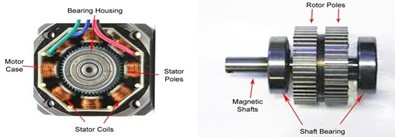
\includegraphics[scale=1]{Chapters/Chapter4/Images/Cautaodongcobuoc.jpg}
\caption{Cấu tạo động cơ bước}
\label{fig:cautaodongcobuoc}
\end{figure}

\subsection{Driver cho động cơ bước}
Một bộ phận không thể thiếu trong điều khiển động cơ bước đó là driver. Driver như là một mạch phân phối xung cho động cơ, làm nhiệm vụ cấp điện cho động cơ bước hoạt động. Có 2 loại driver được xử dụng khá nhiều trong thị trường hiện tại đó là : TB6600 và A4988.

\begin{figure}[ht]
\subfloat[Driver TB6600]
  {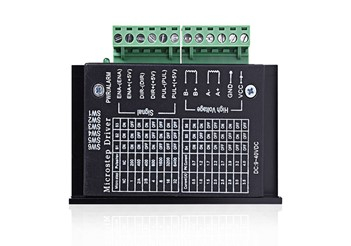
\includegraphics[width=.6\linewidth]{Chapters/Chapter4/Images/DriverTB6600}}\hfill
\subfloat[Driver A4988]
  {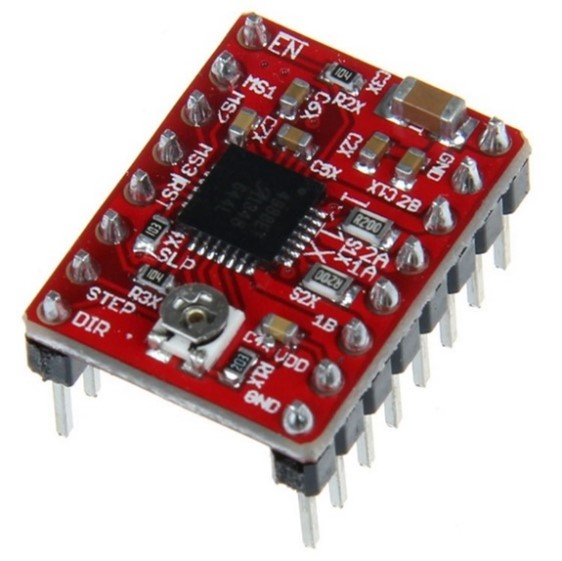
\includegraphics[width=.4\linewidth]{Chapters/Chapter4/Images/DriverA4988}}
\caption{Một số driver cho động cơ bước}
\label{fig:2drivermotor}
\end{figure}

\begin{table}
\centering
\begin{tabular}{|c|c|c|}
\hline 
 & TB6600 & A4988 \\ 
\hline 
Dòng điện ngõ ra & $ 0.5A-4A $ & $ 0.5 - 2A $ \\ 
\hline 
Vi bước nhỏ nhất & $ 1/64 $ & $ 1/16 $ \\ 
\hline 
Điện áp điều khiển & $ 3.3V - 24V $ & $ 0.3V - 5.5V $ \\ 
\hline 
Nguồn cấp cho driver & $ 9V - 42V $ & $ 8V - 35V $ \\ 
\hline 
Bảo vệ quá nhiệt & Có & Có \\ 
\hline 
Bảo vệ ngắn mạch & Có & Không \\ 
\hline 
Kích thước & $ 96 \times 71 \times 37 (mm) $ & $ 5 \times 5 \times 0.9 (mm) $ \\ 
\hline 
Giá thành & 140.000VND & 25.000VND \\ 
\hline 
\end{tabular} 
\caption{Bảng so sánh driver TB6600 và A4988}
\label{tab:sosanhdriver}
\end{table}

Từ Bảng \ref{tab:sosanhdriver}, ta thấy tuy giá thành cao hơn, nhưng driver TB6600 có độ phân giải bước cao hơn, dòng điện điều khiển ngõ ra cũng lớn hơn đồng nghĩa với việc TB6600 sẽ điều khiển vị trí chính xác hơn và động cơ sẽ có momen lớn hơn. Vì thế, trong đồ án này ta sử dụng driver TB6600.

Thông số kỹ thuật:
\begin{itemize}
\item IC Driver: TB6600HQ/HG Single-chip bipolar sinusoidal micro-step stepping motor driver, công nghệ mới nhất BiCD 0.13nm.
\item Nguồn cấp tối đa: 40VDC.
\item Dòng cấp $IIN\_MAX = 5.0A$ và  dòng ra $IOUT\_MAX = 4$.
\item Độ phân giải: 1/1, 1/2, 1/4, 1/8, 1/16, 1/32 và 1/64.
\item Kích thước: 96 x 57 x 35mm.
\end{itemize}

Cách kết nối:
\begin{itemize}
\item DC+: Nối với nguồn điện từ 9 - 40VDC
\item DC- : Điện áp (-) âm của nguồn
\item A+ và A -: Nối vào cặp cuộn dây của động cơ bước
\item B+ và B- : Nối với cặp cuộn dây còn lại của động cơ
\item PUL+: Tín hiệu cấp xung điều khiển tốc độ (+5V) từ BOB cho M6600
\item PUL-: Tín hiệu cấp xung điều khiển tốc độ (-) từ BOB cho M6600
\item DIR+: Tín hiệu cấp xung đảo chiều (+5V) từ BOB cho M6600
\item DIR-: Tín hiệu cấp xung đảo chiều (-) từ BOB cho M6600
\item ENA+ và ENA -: khi cấp tín hiệu cho cặp này động cơ sẽ không có lực momen giữ và quay nữa
\item Có thể đấu tín hiệu dương (+) chung hoặc tín hiệu âm (-) chung.
\end{itemize}


\subsection{Mạch cầu H đầy đủ L298N}
\begin{figure}
\centering
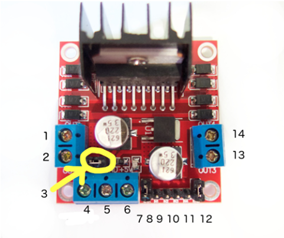
\includegraphics[scale=1]{Chapters/Chapter4/Images/L298N}
\caption{Module L298N}
\label{fig:L298N}
\end{figure}

Thông số kỹ thuật:
\begin{itemize}
\item Driver: L298N tích hợp hai mạch cầu H
\item Điện áp điều khiển: $+5V \sim +12V$
\item Dòng tối đa cho mỗi cầu H là: 2A
\item Điện áp của tín hiệu điều khiển: $ +5V \sim +7V $
\item Dòng của tín hiệu điều khiển : $ 0 \sim 36mA $
\item Công suất hao phí : $ 20W $ (khi nhiệt độ $ T = 75^{\circ}C $)
\item Nhiệt độ bảo quản : $ -25^{\circ}C \sim +130^{\circ}C $
\end{itemize}

Các chân tín hiệu quan trọng:
\begin{itemize}
\item 3: 12V jumper, tháo jumper ra nếu sử dụng nguồn trên 12V. Jumper này dùng để cấp nguồn cho IC ổn áp tạo ra nguồn 5V nếu nguồn trên 12V sẽ làm cháy IC nguồn.
\item 4: Cắm dây nguồn cung cấp điện áp cho motor vào đây từ 6V đến 35V.
\item 5: Cắm chân GND của nguồn vào đây.
\item 6: Ngõ ra nguồn 5V, nếu jumper đầu vào không rút ra.
\item 7: Chân Enable , chân này dùng để cấp xung PWM nếu dùng VDK thì rút jumper ra và cắm chân PWM vào đây.
\item 8, 9, 10, 11: lần lượt là các chân IN1, IN2, IN3, IN4.
\item 12: Chân Enable , chân này dùng để cấp xung PWM nếu dùng VDK thì rút jumper ra và cắm chân PWM vào đây.
\end{itemize}

\subsection{Kit STM32F411 - Discovery}
Thông số kỹ thuật:
\begin{itemize}
\item Bộ điều khiển STM32F411VET6 có 512KB bộ nhớ Flash, 128KB RAM trong gói LQFP100.
\item Cấp nguồn : Thông qua bus USB hoặc cấp điện áp 5V từ bên ngoài.
\item IC L3GD20: Cảm biến chuyển động ST MEMS 3-trục, đầu ra kĩ thuật số.
\item IC LSM303DLHC: Hệ thống ST MEMS trong hệ thống bao gồm bộ cảm biến gia tốc tuyến tính kỹ thuật số 3D và cảm biến từ tính số 3 chiều
\item IC MP45DT02: Bộ cảm biến âm thanh ST MEMS, micro kỹ thuật số.
\item IC CS43L22 : âm thanh DAC với trình điều khiển loa lớp tích hợp D.
\end{itemize}

\begin{figure}[ht]
\centering
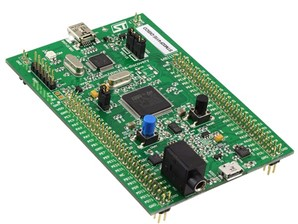
\includegraphics[scale=1]{Chapters/Chapter4/Images/STM32F4.jpg}
\caption{Kit STM32F411 Discovery}
\label{fig:stm32f4}
\end{figure}

\subsection{Module mở rộng giao tiếp I2C 8 kênh TCA9548A}
Thông số kỹ thuật:
\begin{itemize}
\item Điện áp hoạt động: 1.65 – 5.5VDC
\item Số kênh mở rộng: 8 kênh
\item Giao tiếp I2C, địa chỉ chọn được từ 0x70 đến 0x77
\item Điện áp giao tiếp: 1.8, 2.5, 3.3, 5VDC
\item Tần số hoạt động: 0 – 400kHz
\end{itemize}

\begin{figure}
\centering
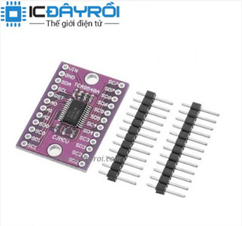
\includegraphics[scale=1]{Chapters/Chapter4/Images/TCA}
\caption{Module TCA9548A}
\label{fig:tca}
\end{figure}


\subsection{PCA9685}
\begin{figure}[htp]
	\centering
	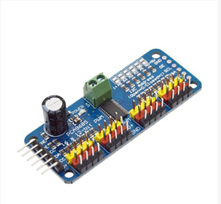
\includegraphics[scale=1]{Chapters/Chapter4/Images/PCA.png}
	\caption{Module PCA9685}
	\label{fig:C4PCA}
\end{figure}
Thông số kỹ thuật:
\begin{itemize}
\item Mạch điều khiển 16 Chanel PWM PCA9685
\item IC chính: PCA9685
\item Điện áp sử dụng: $2.3 \sim 5.5VDC$.
\item Số kênh PWM: 16 kênh, tần số: $40 \sim 1000Hz$
\item Độ phân giải PWM: 12bit.
\item Giao tiếp: I2C (chấp nhận mức Logic TTL $ 3 \sim 5VDC$)
\item Kích thước: $ 62.5mm \times 25.4mm \times 3mm $
\end{itemize}


\subsection{LED công suất 3W}
\begin{figure}[htp]
	\centering
	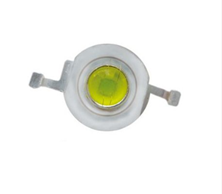
\includegraphics[scale=1]{Chapters/Chapter4/Images/Led3W.png}
	\caption{LED công suất 3W}
	\label{fig:C43W}
\end{figure}
Thông số kỹ thuật:
\begin{itemize}
\item Công suất tiêu thụ 3W
\item Điện áp hoạt động : 3.5-4V
\item Dòng tiêu thụ: 600-750mA
\item Độ sáng : 180LM-200LM
\item Nhiệt độ hoạt động: $ -20^{\circ}C \sim 60^{\circ}C $ \end{itemize}

\subsection{Cảm biến ánh sáng}
Cảm biến cường độ ánh sáng GY-30 BH1750FVI là một cảm biến ánh sáng kỹ thuật số. Gồm một linh kiện điện tử IC cảm biến ánh sáng cho giao tiếp I2C. IC này là thích hợp nhất để nhận diện các dữ liệu ánh sáng xung quanh cho việc điều chỉnh màn hình LCD và bàn phím đèn nền sức mạnh của điện thoại di động. Nó có thể phát hiện nhiều ở độ phân giải cao (1-65535 lx).
\begin{figure}[ht]
	\centering
	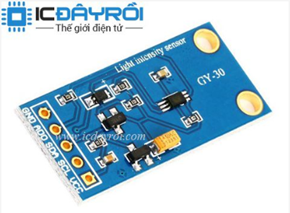
\includegraphics[scale=1]{Chapters/Chapter4/Images/Cambien.png}
	\caption{Cảm biến ánh sáng GY-30 BH1750}
	\label{fig:Cambiengy}
\end{figure}

Thông số kỹ thuật:
\begin{itemize}
\item Module cảm biến cường độ sáng sử dụng chíp BH1750FVI.
\item Điện áp cung cấp: $ 3V - 5V $.
\item Phạm vi phát hiện sáng: $ 0 - 65535 lux $.
\item Cảm biến sử dụng bộ chuyển đổi ADC 16 bit. Tín hiệu đầu ra là tín hiệu số.
\item Giao tiếp với MCU theo chuẩn I2C.
\end{itemize}

\section{Sơ đồ kết nối}

\subsection{Sơ đồ kết nối tổng quát}
Sơ đồ nguyên lý: Hình~\ref{fig:C4Sodotongquat}.

Sơ đồ thực tế: Hình~\ref{fig:C4Sodothucte}.

\begin{figure}[htp]
	\centering
	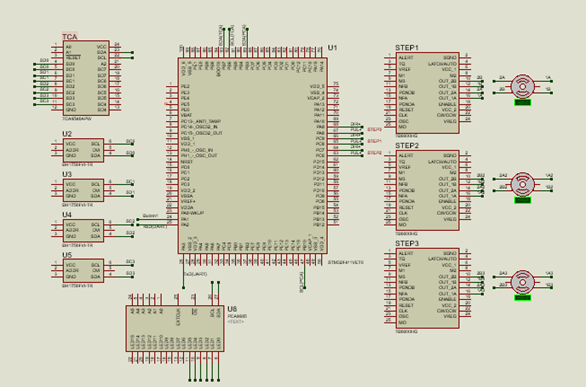
\includegraphics[scale=1]{Chapters/Chapter4/Images/Sodonguyenlytongquat.png}
	\caption{Sơ đồ nguyên lý tổng quát}
	\label{fig:C4Sodotongquat}
\end{figure}
\begin{figure}[htp]
	\centering
	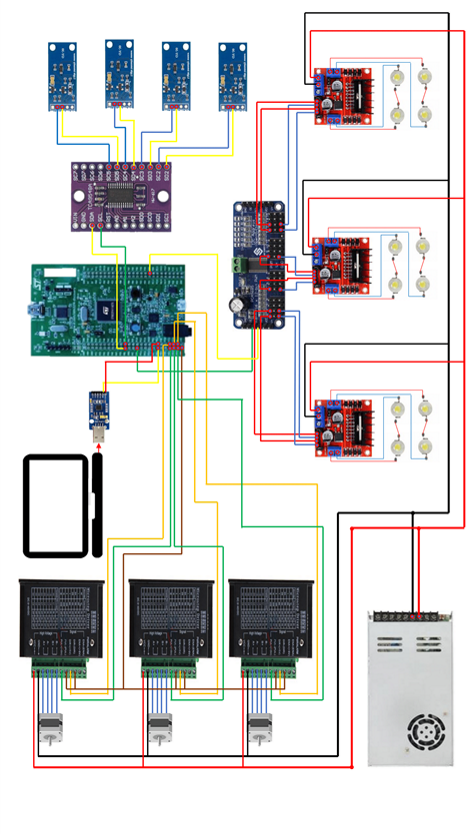
\includegraphics[scale=1]{Chapters/Chapter4/Images/Sodoketnoithucte.png}
	\caption{Sơ đồ kết nối điện thực tế}
	\label{fig:C4Sodothucte}
\end{figure}

\subsection{Sơ đồ kết nối đèn và module L298N}
Sơ đồ nguyên lý: Hình~\ref{fig:C4NLDenL298N}.

Sơ đồ thực tế: Hình~\ref{fig:C4RealDenL298N}.
\begin{figure}[htp]
	\centering
	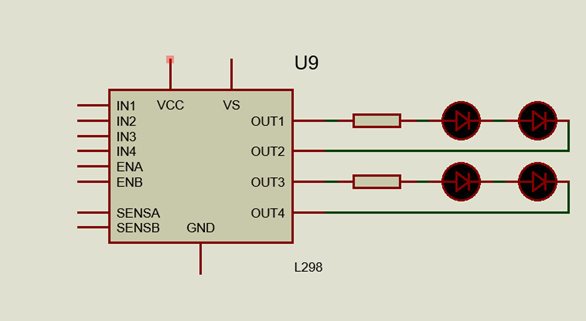
\includegraphics[scale=1]{Chapters/Chapter4/Images/DenL298N.png}
	\caption{Sơ đồ nguyên lý kết nối đèn với module L298N}
	\label{fig:C4NLDenL298N}
\end{figure}
\begin{figure}[htp]
	\centering
	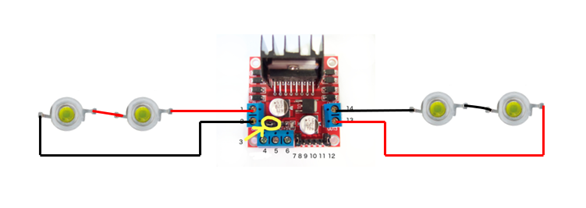
\includegraphics[scale=1]{Chapters/Chapter4/Images/RealDenL298N.png}
	\caption{Sơ đồ kết nối thực tế đèn với module L298N}
	\label{fig:C4RealDenL298N}
\end{figure}

\subsection{Sơ đồ kết nối Driver TB6600 với động cơ bước}
Sơ đồ nguyên lý: Hình~\ref{fig:C4NLDriverDC}.

Sơ đồ thực tế: Hình~\ref{fig:C4RealDriverDC}.

\begin{figure}[htp]
	\centering
	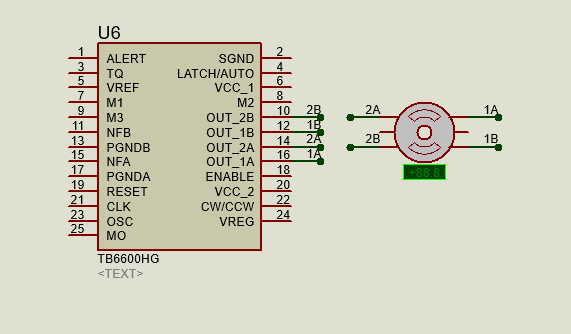
\includegraphics[scale=1]{Chapters/Chapter4/Images/DriverDongco.png}
	\caption{Sơ đồ nguyên lý kết nối Driver và động cơ}
	\label{fig:C4NLDriverDC}
\end{figure}
\begin{figure}[htp]
	\centering
	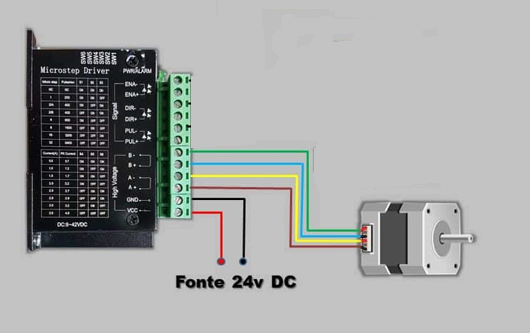
\includegraphics[scale=1]{Chapters/Chapter4/Images/RealDriverDongco.png}
	\caption{Sơ đồ kết nối thực tế Driver và động cơ}
	\label{fig:C4RealDriverDC}
\end{figure}
